% research/paper/paper.tex — V4.3 W11 §79
% LaTeX wrapper for research/paper/paper.md (same content, publication artifact).
% Compile with pdflatex or xelatex; figures under ./figures/, tables under ./tables/.
\documentclass[11pt,a4paper]{article}
\usepackage[utf8]{inputenc}
\usepackage{hyperref}
\usepackage{graphicx}
\usepackage{booktabs}
\usepackage{amsmath}
\usepackage{geometry}
\geometry{margin=1in}
\title{Data Science Agent: An Evidence-Grounded Autonomous Platform for Reproducible Data Science}
\author{Data Science Agent Contributors}
\date{2026-08-31 (V4.3 artifact; reproducibility at \texttt{research/v4\_3/reproducibility/README.md})}
\begin{document}
\maketitle

% The authoritative content is research/paper/paper.md (markdown). This LaTeX
% file provides a print-ready wrapper that \texttt{\textbackslash input}s the
% markdown-derived sections when pandoc is available, or otherwise points the
% reader to the markdown source (the paper's claim→evidence mapping lives there).
% For camera-ready, re-derive this file from paper.md via:
%   pandoc research/paper/paper.md -o research/paper/paper.tex --bibliography=research/paper/references.bib

\noindent\textbf{Note:} This artifact ships as markdown (\texttt{paper.md}) plus this LaTeX wrapper. The markdown is the
canonical source (tables/figures under \texttt{research/paper/\{figures,tables,appendix\}/} are generated from
\texttt{benchmarks/external/datascibench/results/raw\_runs.json} via \texttt{research/v4\_3/generate\_phase\_f\_results.py}); the wrapper exists so a PDF build stays
reproducible without hand edits (\S48).

See \texttt{research/paper/paper.md} for Sections 1--14 (Abstract; Introduction; Related Work; System Design;
Evidence-Grounded Architecture; Evaluation Methodology; Internal Benchmark; External Benchmarks; Real-World Case Studies;
Ablation; Reliability \& Failure Analysis; Reproducibility; Human Evaluation; Limitations; Conclusion) and
\texttt{research/paper/references.bib} for the three cited works (DataSciBench pre-print + repo pin, DSA repo, DSAgentBench).

\begin{figure}[h]
\centering
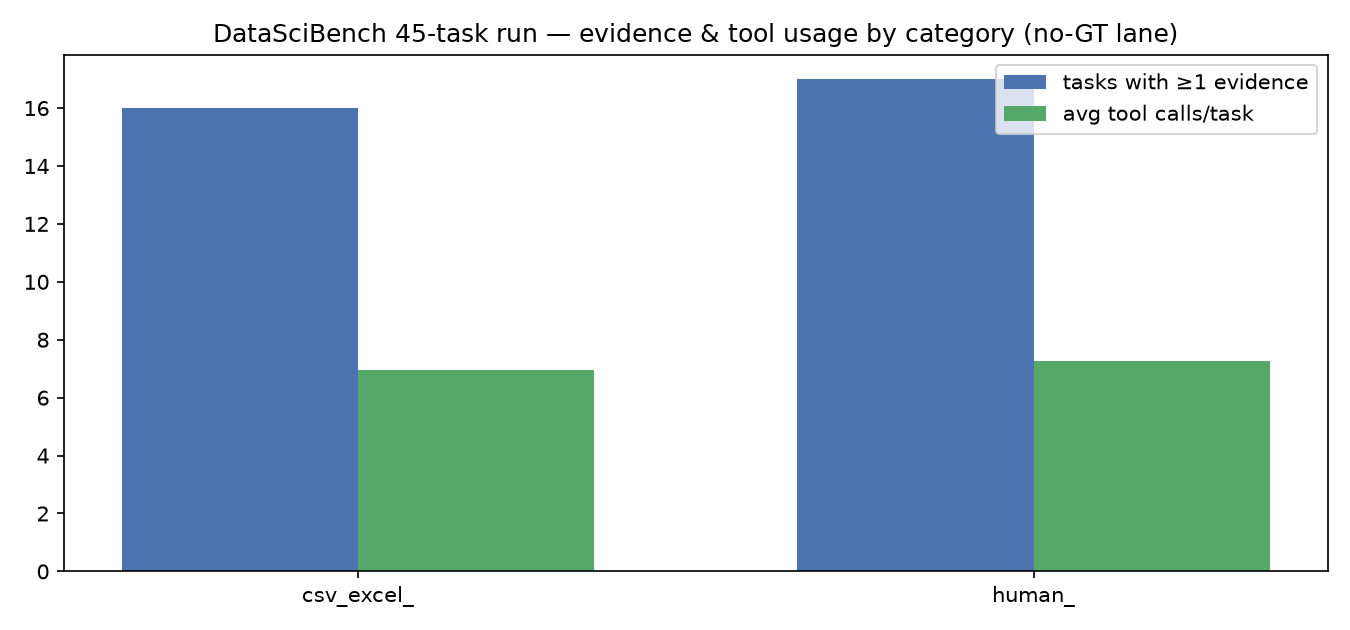
\includegraphics[width=0.9\linewidth]{figures/category_evidence.png}
\caption{Category vs evidence (DataSciBench execution lane; GT absent, no score).}
\end{figure}

\begin{figure}[h]
\centering
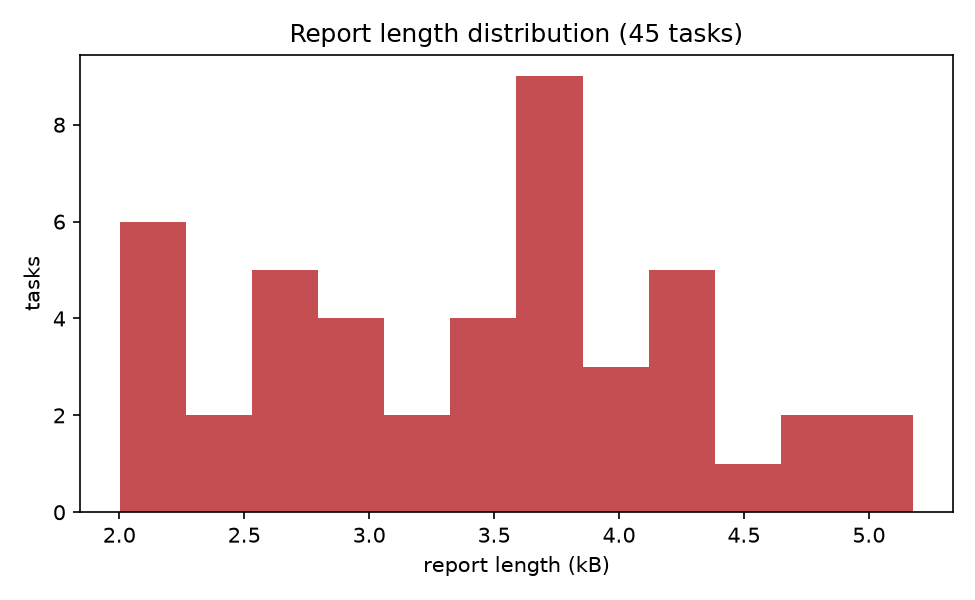
\includegraphics[width=0.9\linewidth]{figures/latency_report.png}
\caption{Latency \& report length (45 runs, median 7 tool calls).}
\end{figure}

\end{document}
